

\chapter{Sprint 5}
\label{Sprint0}
\lhead{Chapter 11. \emph{Sprint 5}}

\section{Duration}
The duration of the sprint was the following:
\begin{itemize}
\item Sprint start:  November, 4th
\item Milestone M3 (feature freeze): November, 4th.
\item Sprint end: November, 20th
\end{itemize}

This sprint was a bit longer than the others because it included the last days
that were left till the end project.

\section{Planning}

The plan for this sprint consisted primarily in report writing and review.
At the beginning of the sprint we arranged with the supervisor to deliver him a mostly finished version of the report by the end of the first week (around Sunday, the 10th) in order to let him give us some last feedback on it.

Regarding the inclusion of Withings in the demonstration scenario, we ultimately dropped it because we had no further time to look into it and we had come to a conclusion that it was not possible for us to fix it.
Furthermore, as already discussed, it would not have hindered the functionality of the product itself.

Since our product was completed on schedule, we were only left some integration and system testing.

\section{Goal(s)}

This was the final sprint of our project. 
Its main goal was to finalize the product and the documentation as well as prepare a presentation.

\section{Results and feedback}

Results for this sprint were largely positive. 
Although there wasn't much time left to complete the report and prepare the presentation, we managed to write quite a lot. 
We sent our supervisor a mostly finished version of our report on the 10th of November. 
He acknowledged our hard work and provided some positive feedback which contributed to further improvements in the quality of the report and motivated the group to keep up the good work. 
He offered to provide more feedback on an updated version of the report, which we submitted on the 17th.

\section{Evaluation}

\begin{figure}
\centering
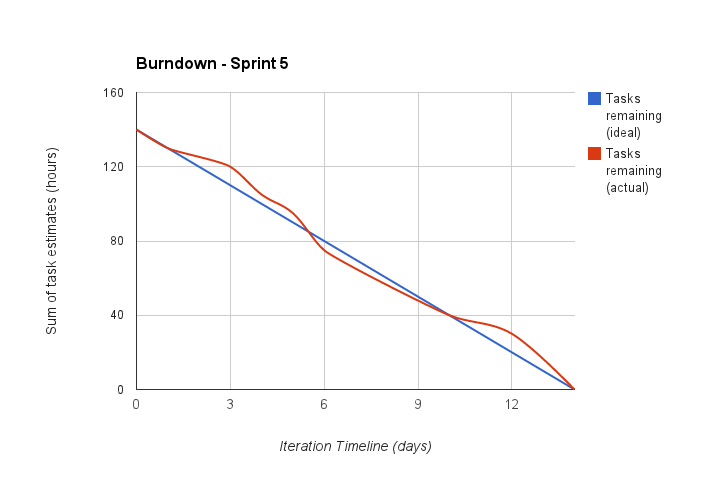
\includegraphics[scale=0.60]{../Figures/burndownSprint5.png}
\caption{Iteration burndown chart}
\label{figure:burndownsprint5}
\end{figure}

The sprint went smoothly. 
The feedback provided by the supervisor was very helpful and helped us to focus our efforts on those parts of the report that were lacking.
Unfortunately some team members were busy with other responsibilities, so the amount of time they could dedicate to the project was somewhat limited.
However, we were still pleased with the quality of the report.

This iteration burndown chart is shown in figure \ref{figure:burndownsprint5}.


\section{Backlog}
See below the sprint backlog.
\begin{enumerate}[1.]
\item \textbf{Project management} included:
	\begin{itemize}
		\item \textbf{Sprint startup meeting}:
			included sprint planning and review
		\item \textbf{Weekly meetings}: 
			meetings with both the customer and the supervisor. Internal meeting with our colleague in Oslo
		\item \textbf{Meeting notes}:
			taking notes during meetings, reviewing of the notes
		\item \textbf{Risk analysis}:
			updated on a weekly basis, so twice per sprint
	\end{itemize}
	\item \textbf{Report work}
		to be done by the team member in Trondheim
	\item \textbf{Additional report work}
		to be done by the team member in Oslo
	\item \textbf{Testing}
		perform integration and system testing
	\item \textbf{Presentation}
		prepare a presentation for the project
\end{enumerate}
